\subsection{Case $r=2$}

Having established the peeling procedure in the simplest setting of $r{=}1$, we now extend the discussion to $r=2$ (removing edges).
This change immediately increases the update complexity of the \cpi: removing a vertex merely shortens a path, whereas removing an edge may remove a path entirely or split it into multiple subpaths.


When an edge $e=\{u,v\}$ that appears on a clique path $\TPath$ is removed from the underlying graph, the effect on $\TPath$ is fully determined by whether $u$ or $v$ are labeled as \emph{\hold} or \emph{\pivot} on this path. We observe the following theorem specifies the update.

\begin{theorem}[Edge Removal]\label{thm:remove_edge}
Let $\TPath=(V_p(\TPath),\,V_h(\TPath))$ be a clique path in the \cpi\ of $G$, and let $e=\{u,v\}$ with $u,v\in V(\TPath)$. For any removed $e$ from $G$,  the updated $\TPath'$ satisfies:

\begin{enumerate}[leftmargin=*]
  \item (\hold-\hold) If $u,v\in V_h(\TPath)$, then $\TPath'=\emptyset$;
  % \item 没主语, if then
  \item (\hold-\pivot) If $u\in V_h(\TPath)$ and $v\in V_p(\TPath)$ (or symmetrically), then
        \[
          \TPath'=\bigl\{\,\bigl(V_p(\TPath)\setminus\{v\},\; V_h(\TPath)\bigr)\,\bigr\};
        \]
  \item (\pivot-\pivot) If $u,v\in V_p(\TPath)$, then
        \[
          \TPath'=\Bigl\{\,
              \bigl(V_p(\TPath)\setminus\{v\},\; V_h(\TPath)\bigr),\;
              \bigl(V_p(\TPath)\setminus\{u\},\; V_h(\TPath)\cup\{v\}\bigr)
            \,\Bigr\}.
        \]
\end{enumerate}

% For all $s$-cliques encoded by $\TPath$ that do not contain $e$, exactly one subpath in $\TPath'$ encodes it.
\end{theorem}

% In all cases, we set $\TPath' = \emptyset$ if $|\TPath'| < s$ according to Lemma~\ref{lem:path_pruning}.

\begin{proof}
We prove the theorem separately for three distinct cases.  
%
(1) If $e$ is a hold-hold edge, every encoded clique would require both endpoints, which becomes impossible after deleting $e$; hence, the path is invalid.  
%
(2) If $e$ is a hold-pivot edge, all encoded cliques must retain the hold endpoint. 
Thus, we update the path with respect to the pivot endpoint, analogous to removing the pivot vertex as described in Lemma~\ref{lem:path_vertex_remove}.  
%
(3) If $e$ is a pivot-pivot edge, we split the path into two:  
(a) $\bigl(V_p(\TPath)\setminus\{v\},\, V_h(\TPath)\bigr)$, which removes all cliques encoded by the path that contain $v$;  
(b) $\bigl(V_p(\TPath)\setminus\{u\},\, V_h(\TPath)\cup\{v\}\bigr)$, which restores all cliques containing $v$ but not $u$.
\end{proof}

\begin{example}
For the \cpi shown in Figure~\ref{fig:pruning_example}, consider the clique path $\TPath{1}$ with
$V_{p}(\TPath{1}) = \{v_4, v_5\}$ and
$V_{h}(\TPath{1}) = \{v_1, v_6\}$.
The three possible updates under edge removal are:

\begin{itemize}[leftmargin=*]
  \item \hold-\hold: Deleting the edge $\{v_1,v_6\}$ removes the entire path, since both endpoints are mandatory.
  \item \hold-\pivot: Deleting the edge $\{v_1,v_4\}$ removes the \pivot $v_4$ from the path while keeping the \hold $v_1$. If the residual path is shorter than $k$, it is discarded.
  \item \pivot-\pivot: Deleting the edge $\{v_4,v_5\}$ splits $\TPath{1}$ into two disjoint paths:
  \[
    \TPath{1.1} : V_{h}(\TPath{1.1}) = \{v_1, v_6\}, \; V_{p}(\TPath{1.1}) = \{v_4\},
  \]
  \[
    \TPath{1.2} : V_{h}(\TPath{1.2}) = \{v_1, v_6, v_5\}, \; V_{p}(\TPath{1.2}) = \emptyset.
  \]
\end{itemize}
\end{example}

% \begin{remark}[Relation to $r=1$]\todo{}
% This theorem uses the same $\hold/\pivot$ invariant as Lemma~\ref{lem:path_vertex_remove}.
% But does not reduce edge removal to vertex removal. In the \hold-\pivot
% case, the \emph{effect on that path} coincides with removing the \pivot
% endpoint as in Lemma~\ref{lem:path_vertex_remove}(2), yet globally $v$ remains
% allowed on other paths where it does not conflict with $u$. The \pivot-\pivot
% split has no counterpart in $r=1$.
% \end{remark}

% \begin{algorithm}[t]
\small
    \small
\caption{\textsc{$(2,s)$-CND}}
\label{alg:peeling_r2}
\KwIn{Succinct Clique Tree (\sct) $\tree$, Clique size $s$}
\KwOut{Core value $\kappa_s(v)$ for every vertex $v$}
\SetKwFunction{RemoveNode}{RemoveNode}
\SetKwFunction{CountPreEdges}{$s$-CliqueCount}
\SetKwProg{Fn}{Function}{:}{}

$count\gets \CountPreEdges(\tree,2,s)$\;

build min heap $H_{\min}$ using $count$\;

$c_{min} \gets 0$\;

\While{$H_{\min}$ is not empty}{
    $e_{min} \gets \text{ExtractMin}(H_{\min})$\;
    $c_{min} \gets \max(c_{min}, count(e_{min}))$\;
    $\kappa_s(e_{min}) \gets c_{min}$\;
    \ForEach{$e \in e_{min}$}{
        % remove edge base on lemma~\ref{lem:remove_edge}
        \ForEach{leaf $\TPath$ containing $e$}{
            \text{Remove Edge $e$ from $\TPath$ based on Theorem~\ref{thm:remove_edge}}\;
        }
    }
    \ForEach{leaf $\TPath$ containing $e \in e_{min}$}{
        Update $count(e')$ and $H_{\min}$ for all edges $e' \in \TPath$
    }  

}

\Return{$\kappa_s(e)$ for all edges $e$}\;

\end{algorithm}

% Based on Theorem~\ref{thm:remove_edge}, we derive the Nuclear Core Decomposition algorithm for the $r=2$ case, as shown in Algorithm~\ref{alg:peeling_r2}. Compared with $r=1$, the $r=2$ case reuses the same peeling pattern; the only changes are that counts are maintained per edge and the local update removes an edge from the affected clique paths.

% \paragraph{Algorithm Description.}
% Algorithm~\ref{alg:peeling_r2} follows the same peeling template as the $r=1$ case with vertices replaced by edges. We first compute, for every edge, its number of $s$-cliques (Lemma~\ref{lem:clique_count}) and build a min-heap keyed by these counts. Iteratively, we extract the minimum $e_{\min}$, set $\kappa_s(e_{\min})$ to the running minimum, and remove $e_{\min}$ from every \cpi leaf that contains it using Theorem~\ref{thm:remove_edge}. We then update the counts and heap entries only for edges that remain on those affected leaves. The loop terminates when the heap becomes empty.

% 与删除节点不同, 批量删除vertex是很简单的, 
\stitle{Batched Updates.}
%
Removing a single edge is straightforward using Theorem~\ref{thm:remove_edge}; 
however, handling batched updates is non-trivial.
%
During the peeling process, multiple edges are often removed simultaneously. 
Processing them sequentially revisits the same paths multiple times, and especially in the \pivot{-}\pivot\ case, each deletion may split a path, causing subsequent removals to cascade across newly created branches. 
%
This makes one-by-one removal prohibitively expensive. 
%
To address this, we adopt a \textit{branch-wise}, \textit{path-local} batched update strategy: for each clique path, we merge all affected edges and update them in a single pass.

% \todo{we resolve all branchings in a single pass by enumerating only its surviving cliques, while cases with a \hold endpoint remain trivial (removing either the entire path or a single node).}

% \stitle{Key Idea.} \todo{}
% 我们的思路是构建当前root-leaf路径的邻接子图, 然后在该邻接子图上计算拆分之后的path.
% Our idea is to construct the adjacency subgraph of the current clique path and then compute the split paths on that subgraph.
% % 
% We observe that the maximum clique sizes are relatively small across different real-world graphs (Table~\ref{tab:maxclique_sizes}). 
% % 这也就意味着CPI中root-leaf路径的长度是较小的
% which implies that the length of clique paths in the \cpi is small. 
% 这使得我们可以在构建adjacency subgraph时使用adjacency bitset.
% Key idea paragraph replacement

\stitle{Key Idea.} 
%
We first handle the simple cases (\hold{-}\hold\ removals delete the entire path, and \hold{-}\pivot\ removals exclude the pivot), before addressing the more complex scenario of removing multiple \pivot{-}\pivot paths simultaneously. 
%
For \pivot{-}\pivot paths, the core idea is to first construct a \textit{residual graph} from vertices in $V(\TPath)$, retaining only the edges that remain valid within this subgraph.
%
We then reconstruct new clique paths from the residual graph. 
Since the residual graph is small (no larger than the maximum clique in the graph), this reconstruction can be performed efficiently, avoiding redundant computation.

% into a small \textit{residual graph} on $V(\TPath)$ and run a pivot-only, path-local search that enumerates precisely the    (all holds plus some pivots), 

% each directly materializing one updated path. 
% This replaces repeated edge-by-edge splits with a single pass and avoids enumerating global $s$-cliques; near-cliques collapse to a single pure-pivot path when possible.
% 
% Bitwise operations enable efficient computation of intersections, counts, and other set operations.

% 我们发现,  构建tree的算法(Algorithm~\ref{alg:buildCPI}})会保证每一个root-leaf都有至少一个keep节点, 这实际上会造成tree不够紧密. 
% 在图Figure~\ref{sec:introduction}中, 节点1 2 3 4 5组成了一个5clique, 这实际上可以简单用单个由5个pivot 组成的root-leaf路径来表示.
% 但是目前的现有的CPI构建算法则需要构建5个path, 分别是$V_{h}(\TPath{1}) = {v_1}$, $V_{p}(\TPath{1}) = {v_2, v_3, v_4, v_5}$. $V_{h}(\TPath{2}) = {v_2}$, $V_{p}(\TPath{2}) = {v_3, v_4, v_5}$. $V_{h}(\TPath{3}) = {v_3}$, $V_{p}(\TPath{3}) = {v_4, v_5}$. $V_{h}(\TPath{4}) = {v_4}$, $V_{p}(\TPath{4}) = {v_5}$. $V_{h}(\TPath{5}) = {v_5}$, $V_{p}(\TPath{5}) = {\emptyset}$.
% Algorithm~\ref{alg:buildCPI} enforces that every clique path contains at least one \hold. This invariant can make the representation less compact: for example, the 5-clique on nodes 1--5 in Figure~\ref{sec:introduction} could be encoded by a single path of five \pivot nodes, yet Algorithm~\ref{alg:buildCPI} materializes one path per choice of \hold. This difference will matter for our update routine.


\begin{algorithm}[t]
\small
\caption{\textsc{UpdateIndex} $(r=2)$}
\label{alg:removeEdge}
\KwIn{clique path $\TPath{} = \{V_{H},V_{P}\}$, remove-edge set $E_{\mathrm{rm}},$ $s > 0$}
\KwOut{All subpaths induced after deleting $E_{\mathrm{rm}}$}
\SetKwFunction{PLBU}{PathUpdate}
\SetKwFunction{BK}{PathUpdate}
\SetKwProg{Fn}{Function}{:}{}

% % 如果包含hold-hold edge，直接删掉整条path
% % $\exists e \in E_{\mathrm{rm}}$ s.t. $e$ is hold-hold edge on $\TPath{}$
% \If{$\exists e \in E_{\mathrm{rm}}$ s.t. $e$ is hold-hold edge on $\TPath{}$}{
%     \Return
% }

% % 对于所有的hold-pivot edge，删掉pivot
% \ForEach{$e=\{u,v\} \in E_{\mathrm{rm}}$ s.t. $e$ is hold-pivot edge on $\TPath{}$}{
%     \If{$u$ is pivot on $\TPath{}$}{remove $u$ from $\TPath{}$}
%     \ElseIf{$v$ is pivot on $\TPath{}$}{remove $v$ from $\TPath{}$}
% }

% hold-hold: drop the entire path
% \If{$\exists\,e\inE_{\mathrm{rm}}:\ e\subseteq V_h(\TPath{})$}{\Return}
% make return one line
\lIf{$\exists\,e\in E_{\mathrm{rm}} :\ e\subseteq V_h(\TPath{})$}{\Return}

% hold-pivot: remove the pivot endpoint
\ForEach{$e\in E_{\mathrm{rm}} :\ |e\cap V_h(\TPath{})|=1$}{
  remove $(e\cap V_p(\TPath{}))$ from $\TPath{}$

  remove $e$ from $E_{\mathrm{rm}}$
  }

% $H \gets$ complete graph on $V(\TPath{})$ with edges in $E_{\mathrm{rm}}$

% OR, if you want the whole line in math mode with text inside:
$H \gets \text{ a residual graph on } V(\TPath{}) \text{ with edges in } E_{\mathrm{rm}} \text{ removed} $

$v_{fixed} \gets \{\,v\in V(H)\mid v \text{ is not incident to any edge of } E_{\mathrm{rm}}\,\}$

$Piv \gets \{\,v\in v_{fixed} \mid v \text{ is a pivot on } \TPath{}\,\}$

$R \gets v_{fixed}$,\quad $P \gets V(H)\setminus v_{fixed}$

\PLBU{$R, P, Piv$}

\Fn{\PLBU{$R,\,P,\,Piv$}}{
  \lIf{$|R \setminus Piv|>s$}{
    \Return
  }
  \If{$P=\emptyset$}{
    \lIf{$|R|\leq s$}{\textbf{output path }$\{R,\,Piv\}$}
    % \textbf{output path }$\{R,\,Piv\}$\;
    \Return
  }
  $u_{piv} \gets \arg\max_{x\in P} |P\cap N_H(x)|$\;
  \ForEach{$v\in P \setminus N_H(u_{piv})$}{
    $R' \gets R \cup \{v\}$;\quad $P' \gets P \cap N_H(v)$\;

    \lIf{$v=u_{piv}$}{$Piv' \gets Piv \cup \{v\}$}
    \lElse{$Piv' \gets Piv$}

    \PLBU{$R',\,P',\,Piv'$}\;

    $P \gets P \setminus \{v\}$\;
  }
}
\end{algorithm}

% \begin{figure*}[t]
%     \centering
%     \includegraphics[width=\textwidth]{figure/newTree.eps}
%     \caption{An example tree produced by the Algorithm~\ref{alg:removeEdge}. White nodes are \pivot vertices, gray nodes are \hold vertices.}
%     \label{fig:new_tree_example}
% \end{figure*}

\begin{figure}[t]
    \centering
    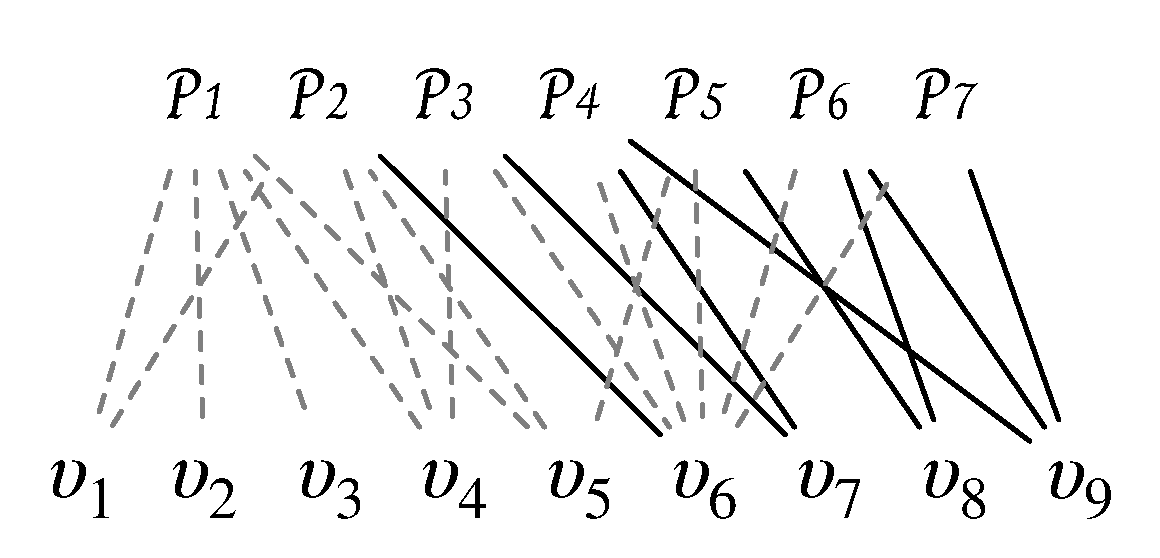
\includegraphics[width=0.30\textwidth]{figure/CPIlarge.eps}
    % 虚线连接的节点是\pivot节点, 实线连接的节点是\hold节点.
    \caption{
        An example of a \cpi on Figure~\ref{fig:graph_example} (no pruning). Dashed nodes denote pivots, and solid nodes denote holds.
    }
    \label{fig:new_tree_example}
\end{figure}

\stitle{Algorithm.} 
% 因此我们提出了一个batched path update的算法(Algorithm~\ref{alg:removeEdge}), 来进行对于一条路径上多个edge的删除.
% The process is listed in Algorithm~\ref{alg:removeEdge}. 
%
The algorithm (Algorithm~\ref{alg:removeEdge}) takes as input a clique path $\TPath$, a set $E_{\mathrm{rm}}$ of edges to remove, and the target clique size $s$ (for pruning). 
It first constructs the residual graph $H$ by deleting all edges in $E_{\mathrm{rm}}$ from the complete graph induced by $V(\TPath)$. 
Next, it identifies the set of \emph{fixed} vertices $V_{\text{fixed}}$ in $H$ that are not incident to any removed edge, and determines the subset of \pivots\ among these fixed vertices. 
The sets $R$ and $P$ are then initialized as $R = V_{\text{fixed}}$ and $P = V(\TPath) \setminus V_{\text{fixed}}$, respectively. 
%
Finally, a recursive Bron-Kerbosch-like search function, \BK, is invoked to enumerate all valid subpaths from the residual graph. 
In each recursive call, a pivot vertex connected to the largest number of vertices in $P$ is selected~\cite{BronKerbosch}, and the search expands along its connected candidates to generate the cliques that define the updated path(s).


\begin{remark}
A question arises as to why Algorithm~\ref{alg:buildCPI} is not directly reused. 
%
Algorithm~\ref{alg:buildCPI} constructs a \emph{\hold-anchored} index, where every clique path must contain at least one \hold. 
However, our focus in Algorithm~\ref{alg:removeEdge} is primarily on updating \pivot{-}\pivot relations. 
The proposed batched path update relaxes this constraint, allowing a path to remain pure-\pivot after updates. 
Permitting pure-\pivot paths preserves the same encoding semantics while producing a more compact index and reducing the number of paths that need to be updated—particularly under frequent \pivot-\pivot\ deletions. 
As illustrated in Figure~\ref{fig:new_tree_example}, a 5-clique can thus be represented by a single pure-\pivot\ path instead of multiple hold-anchored duplicates.
\end{remark}

% 在实现上, 我们使用bitset(Definition~\ref{def:bitset})来表示路径上的节点集合, 以加速集合交集和计数等操作.
\stitle{Implementation.}
The size of the residual graph is bounded by the maximum clique size of the input graph, which is typically small for real-world datasets (Table~\ref{tab:graph-stats}). 
This allows us to represent the residual graph as an adjacency matrix and employ \emph{bitsets} to encode vertex sets on paths, enabling highly efficient set operations (\textsc{and}, \textsc{or}, \textsc{xor}, \textsc{count}) through word-level parallelism~\cite{bitsetClique}. This optimization also applies to cases with $r \ge 3$.


% \begin{definition}[Bitset]\label{def:bitset}
% Given an ordered vertices list $[v_0,$ $\ldots,v_{n-1}]$, a \emph{bitset of length $n$} is the vector $b_{n-1}\ldots b_0$ with $b_i=1$ iff $v_i$ is selected, or $0$ otherwise. Word-level operations (\textsc{and}, \textsc{or}, \textsc{xor}, \textsc{count}) run in constant time and are highly efficient when $n$ is at most a few hundred.

% 该算法的正确性由以下定理来保证. 
% The following theorem guarantees the correctness of the Algorithm \ref{alg:removeEdge}.
\stitle{Correctness.} 
The correctness of cases (1) and (2) is straightforward. 
For case (3), since all \pivot{-}\pivot\ edges marked for removal are deleted from the residual graph, no clique containing any removed edge can be encoded by the reconstructed paths. 
Meanwhile, all remaining edges from the original clique path are preserved in the residual graph. 
Applying the Bron-Kerbosch search~\cite{Pivoter} on the residual subgraph ensures that all surviving cliques are correctly and uniquely encoded by the new paths.




\stitle{Complexity.} 
Let a clique path $\TPath = \{V_p(\TPath), V_h(\TPath)\}$.
Let $L=|V_h(\TPath)|+|V_p(\TPath)|$ and let $\omega_H$ be the maximum clique size in the residual graph $H$ on $V(\TPath)$. If a hold-hold edge exists, we return in $O(1)$ time. Otherwise the preprocessing on the path is linear, and the only non-trivial part is the local Bron-Kerbosch-like search on $H$, which costs $O(3^{\,\omega_H/3})$ time with $O(L^2)$ extra space.